\documentclass[9pt]{beamer}

\usepackage{booktabs}
\usepackage{geometry}
\usepackage{enumitem}

\usetheme{Copenhagen}

\title{Knowledge Grounding in Retrieval-Augmented LMs \\ Quick Update}
\author{Martin Fixman et. al}
\institute{City, University of London}
\date{30 August 2024}

\begin{document}

\begin{frame}
	\titlepage{}
\end{frame}

\section{What's new}
\begin{frame}{New questions}
	More questions were added, including:

	\begin{itemize}
		\item What was the duration of \texttt{\{historical\_event\}}?
		\item What are the dimensions of \texttt{\{painting\}}?
		\item What is the melting point of \texttt{\{element\}}?
		\item What's the main nationality of \texttt{\{person\}}?
	\end{itemize}
\end{frame}

\begin{frame}{New Questions}
	\centering
	\begin{tabular}{r r c r c r}
		\toprule
		Category & Questions & & Objects & & Total \\
		\midrule
		\texttt{book} & 5 & + & 45 & = & 225 \\
		\texttt{city} & 7 & + & 60 & = & 420 \\
		\texttt{element} & 5 & + & 35 & = & 175 \\
		\texttt{historical\_event} & 3 & + & 56 & = & 168 \\
		\texttt{painting} & 7 & + & 39 & = & 273 \\
		\texttt{person} & 7 & + & 47 & = & 329 \\
		\texttt{principle} & 5 & + & 30 & = & 150 \\
		\midrule
		Total & 39 & & 312 & & 2040
		\bottomrule
	\end{tabular}
\end{frame}

\begin{frame}{Better calculation of probabilities}
	Now we properly use\footnotemark{} perplexity rather than average-of-token-probabilities.

	\begin{align*}
		\text{CE} &= - \frac{1}{N} \sum \log P(x_i) \\
		\text{Perplexity} &= e ^ {\text{CE}}
	\end{align*}

	\pause{}

	\footnotetext{Due to a last-minute problem with precision on some large answers, today's plots will still have average-of-token-probabilities. Sorry!}.
\end{frame}

\begin{frame}{Different flavour of Llama}
	Part of the hypothesis\footnotemark{}.

	\vfill{}

	\begin{center}
		\begin{Large}
			Will a larger model tend to prefer parametric answers?
		\end{Large}
	\end{center}

	\vfill{}

	I'm not using two models of Llama:
	\begin{itemize}
		\item \texttt{meta-llama/Meta-Llama-3.1-8B-Instruct}
		\item \texttt{meta-llama/Meta-Llama-3.1-70B-Instruct}
	\end{itemize}

	More models will come soon!

	\footnotetext{The full hypothesis will come later.}
\end{frame}

\begin{frame}
	Calculating probabilities for both parametric and counterfactual answer, regardless of which one gets answered.

	\vfill{}

	\centering
	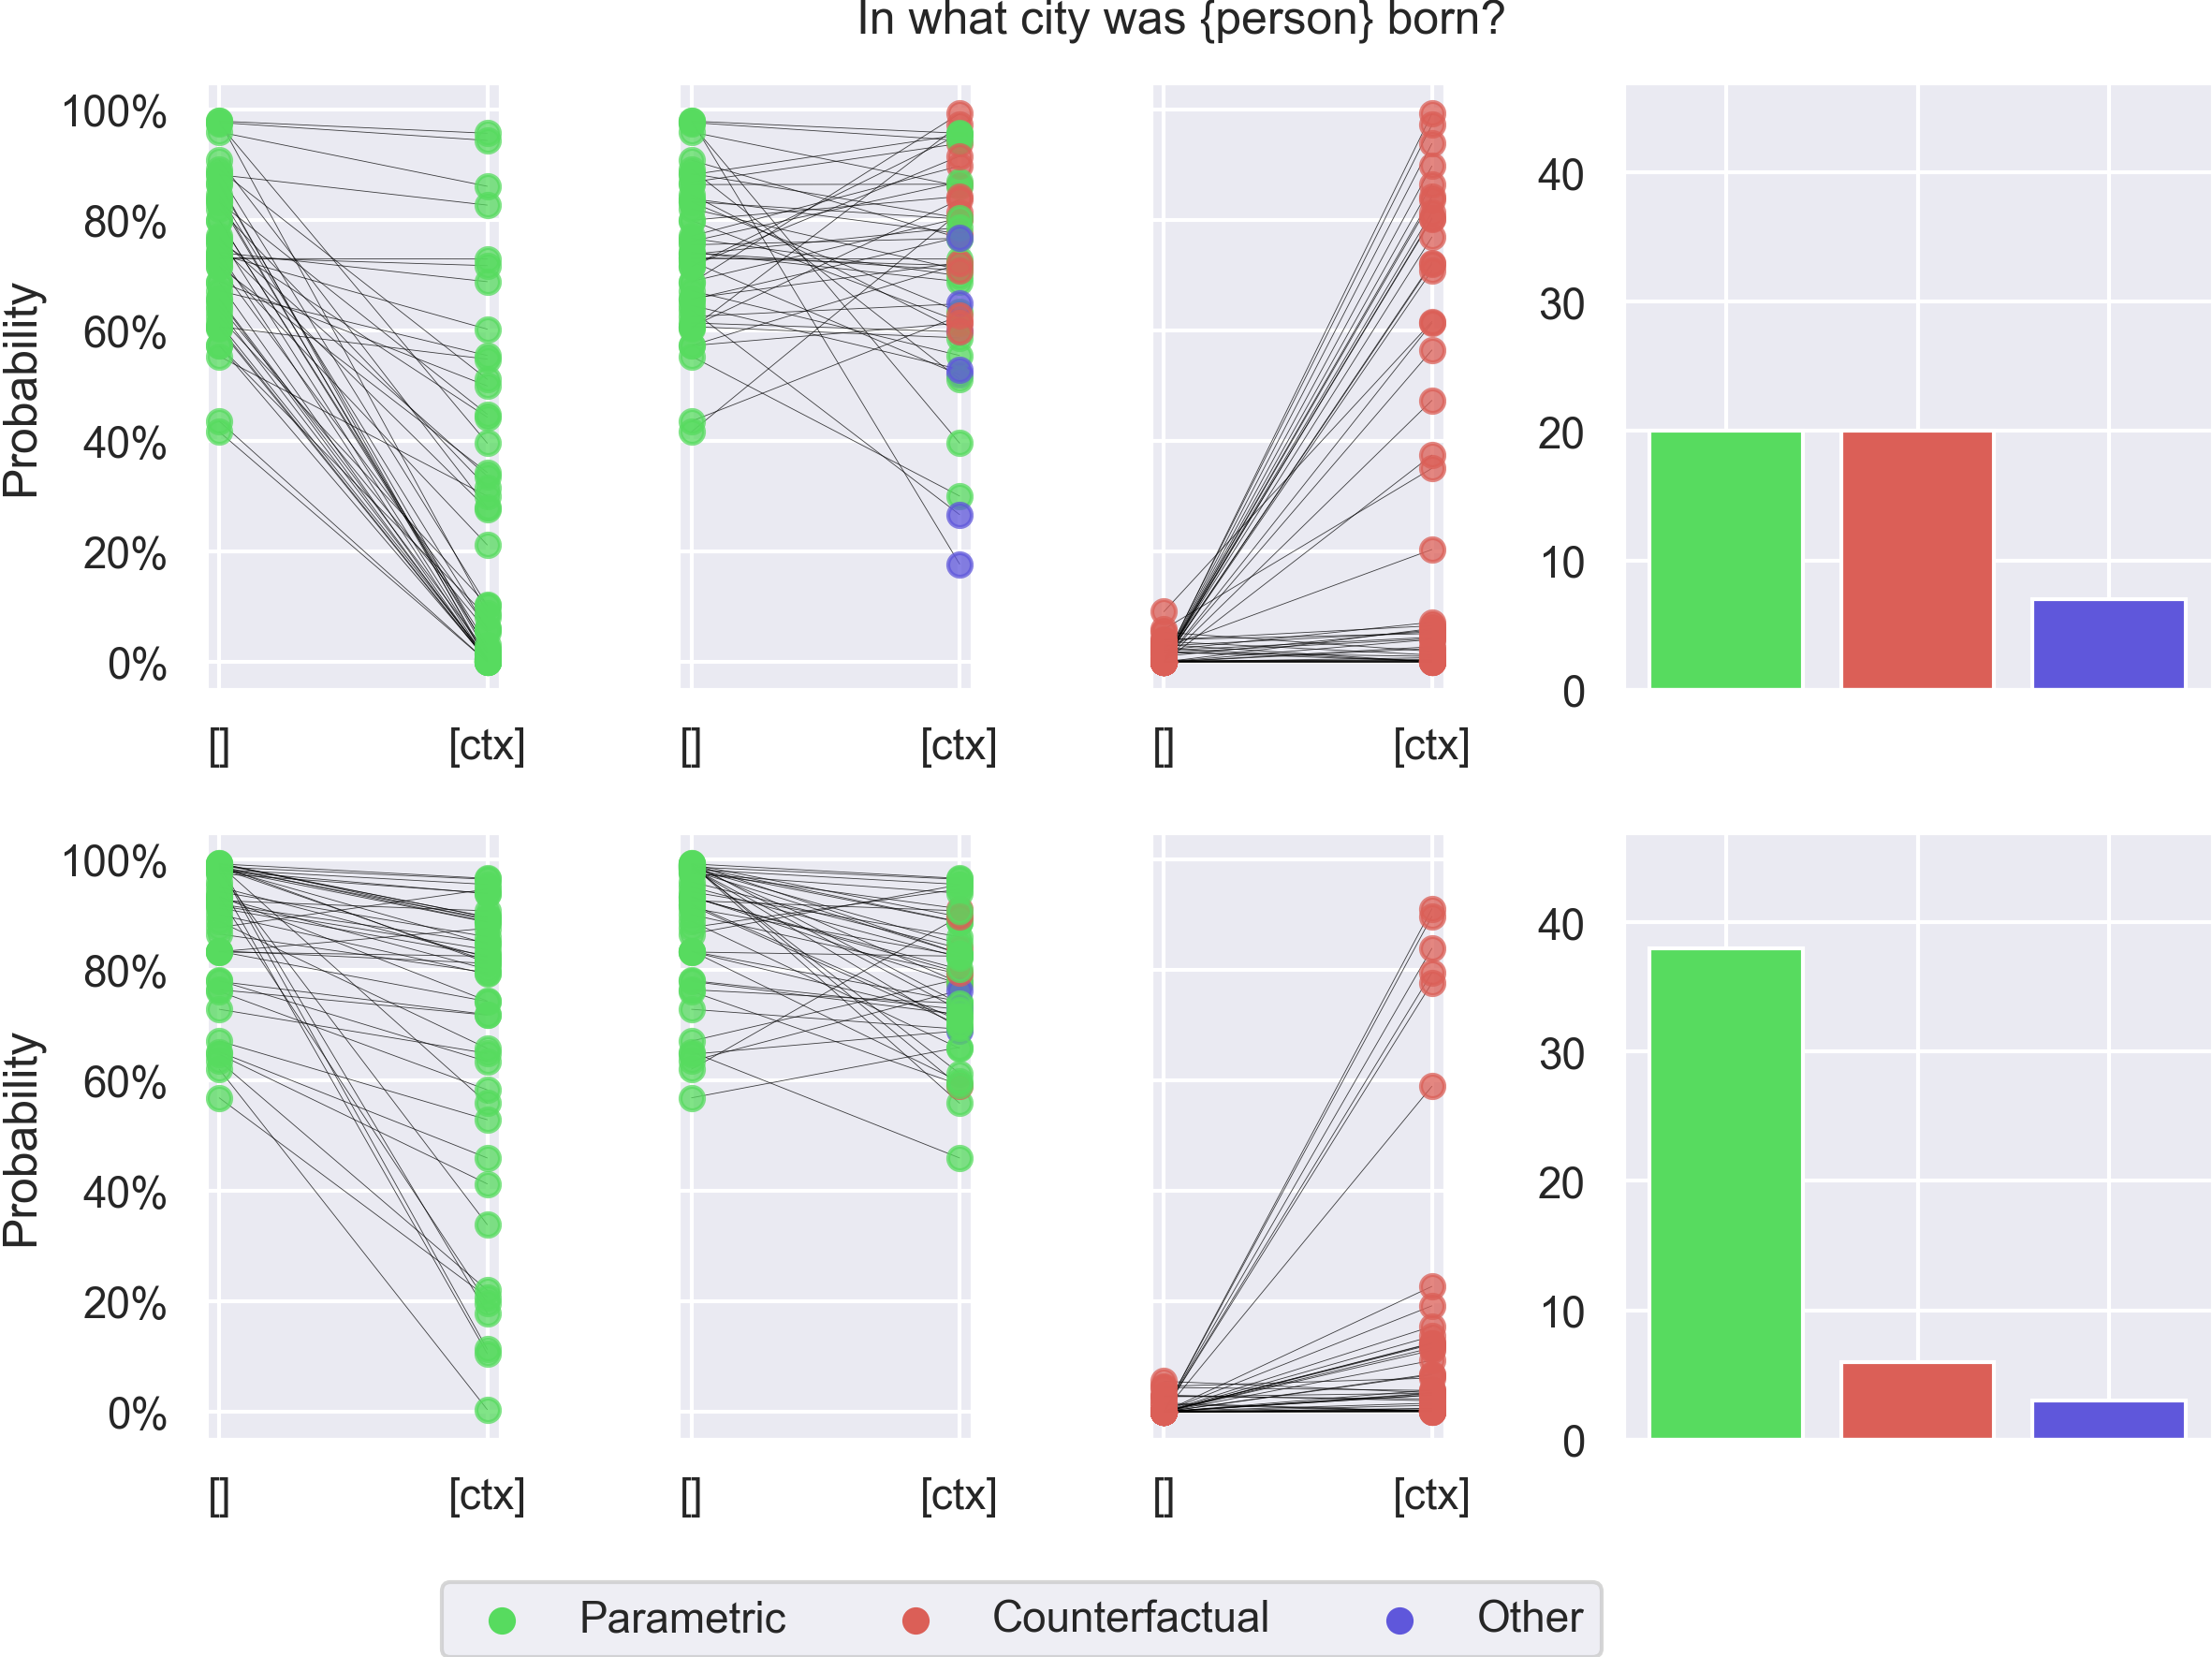
\includegraphics[width=.8\textwidth]{../figures/llama_47.png}
\end{frame}

\section{Some interesting results}
\begin{frame}{Some interesting results}
	Larger models tend to have a higher chance of choosing a parametric answer when given counterfactual information.

	\vfill{}

	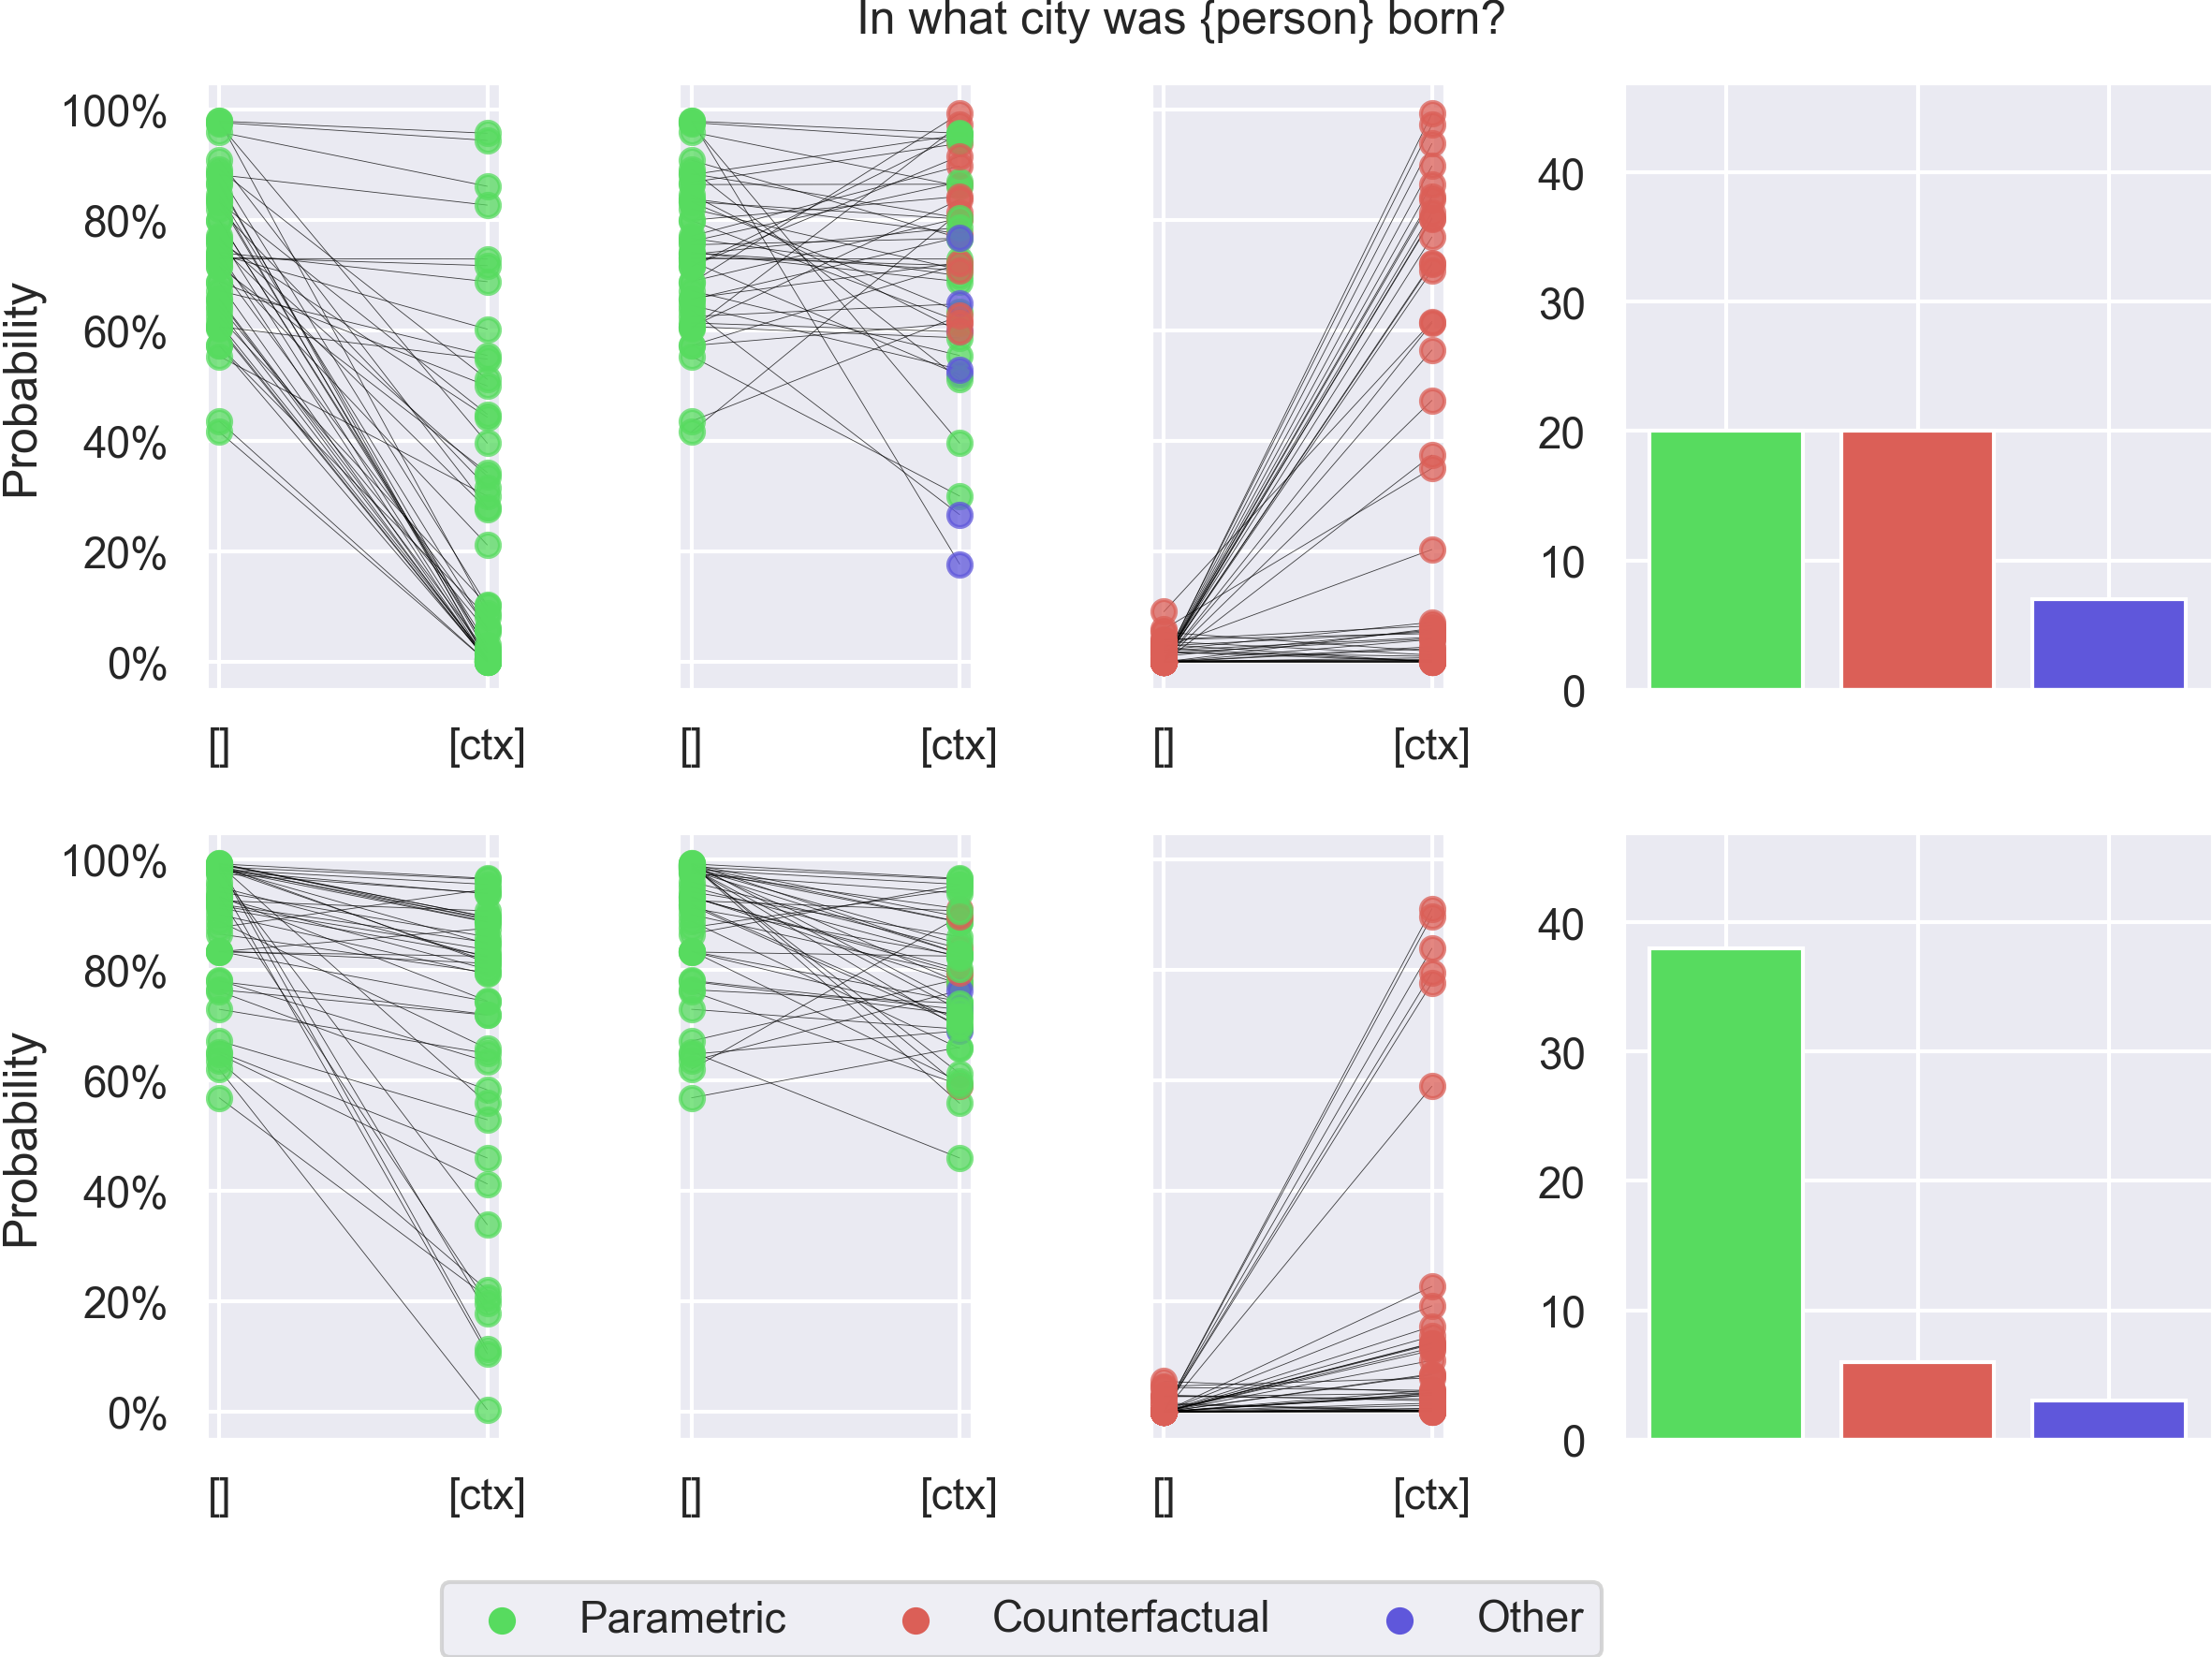
\includegraphics[width=.4\textwidth]{../figures/llama_47.png} \qquad
	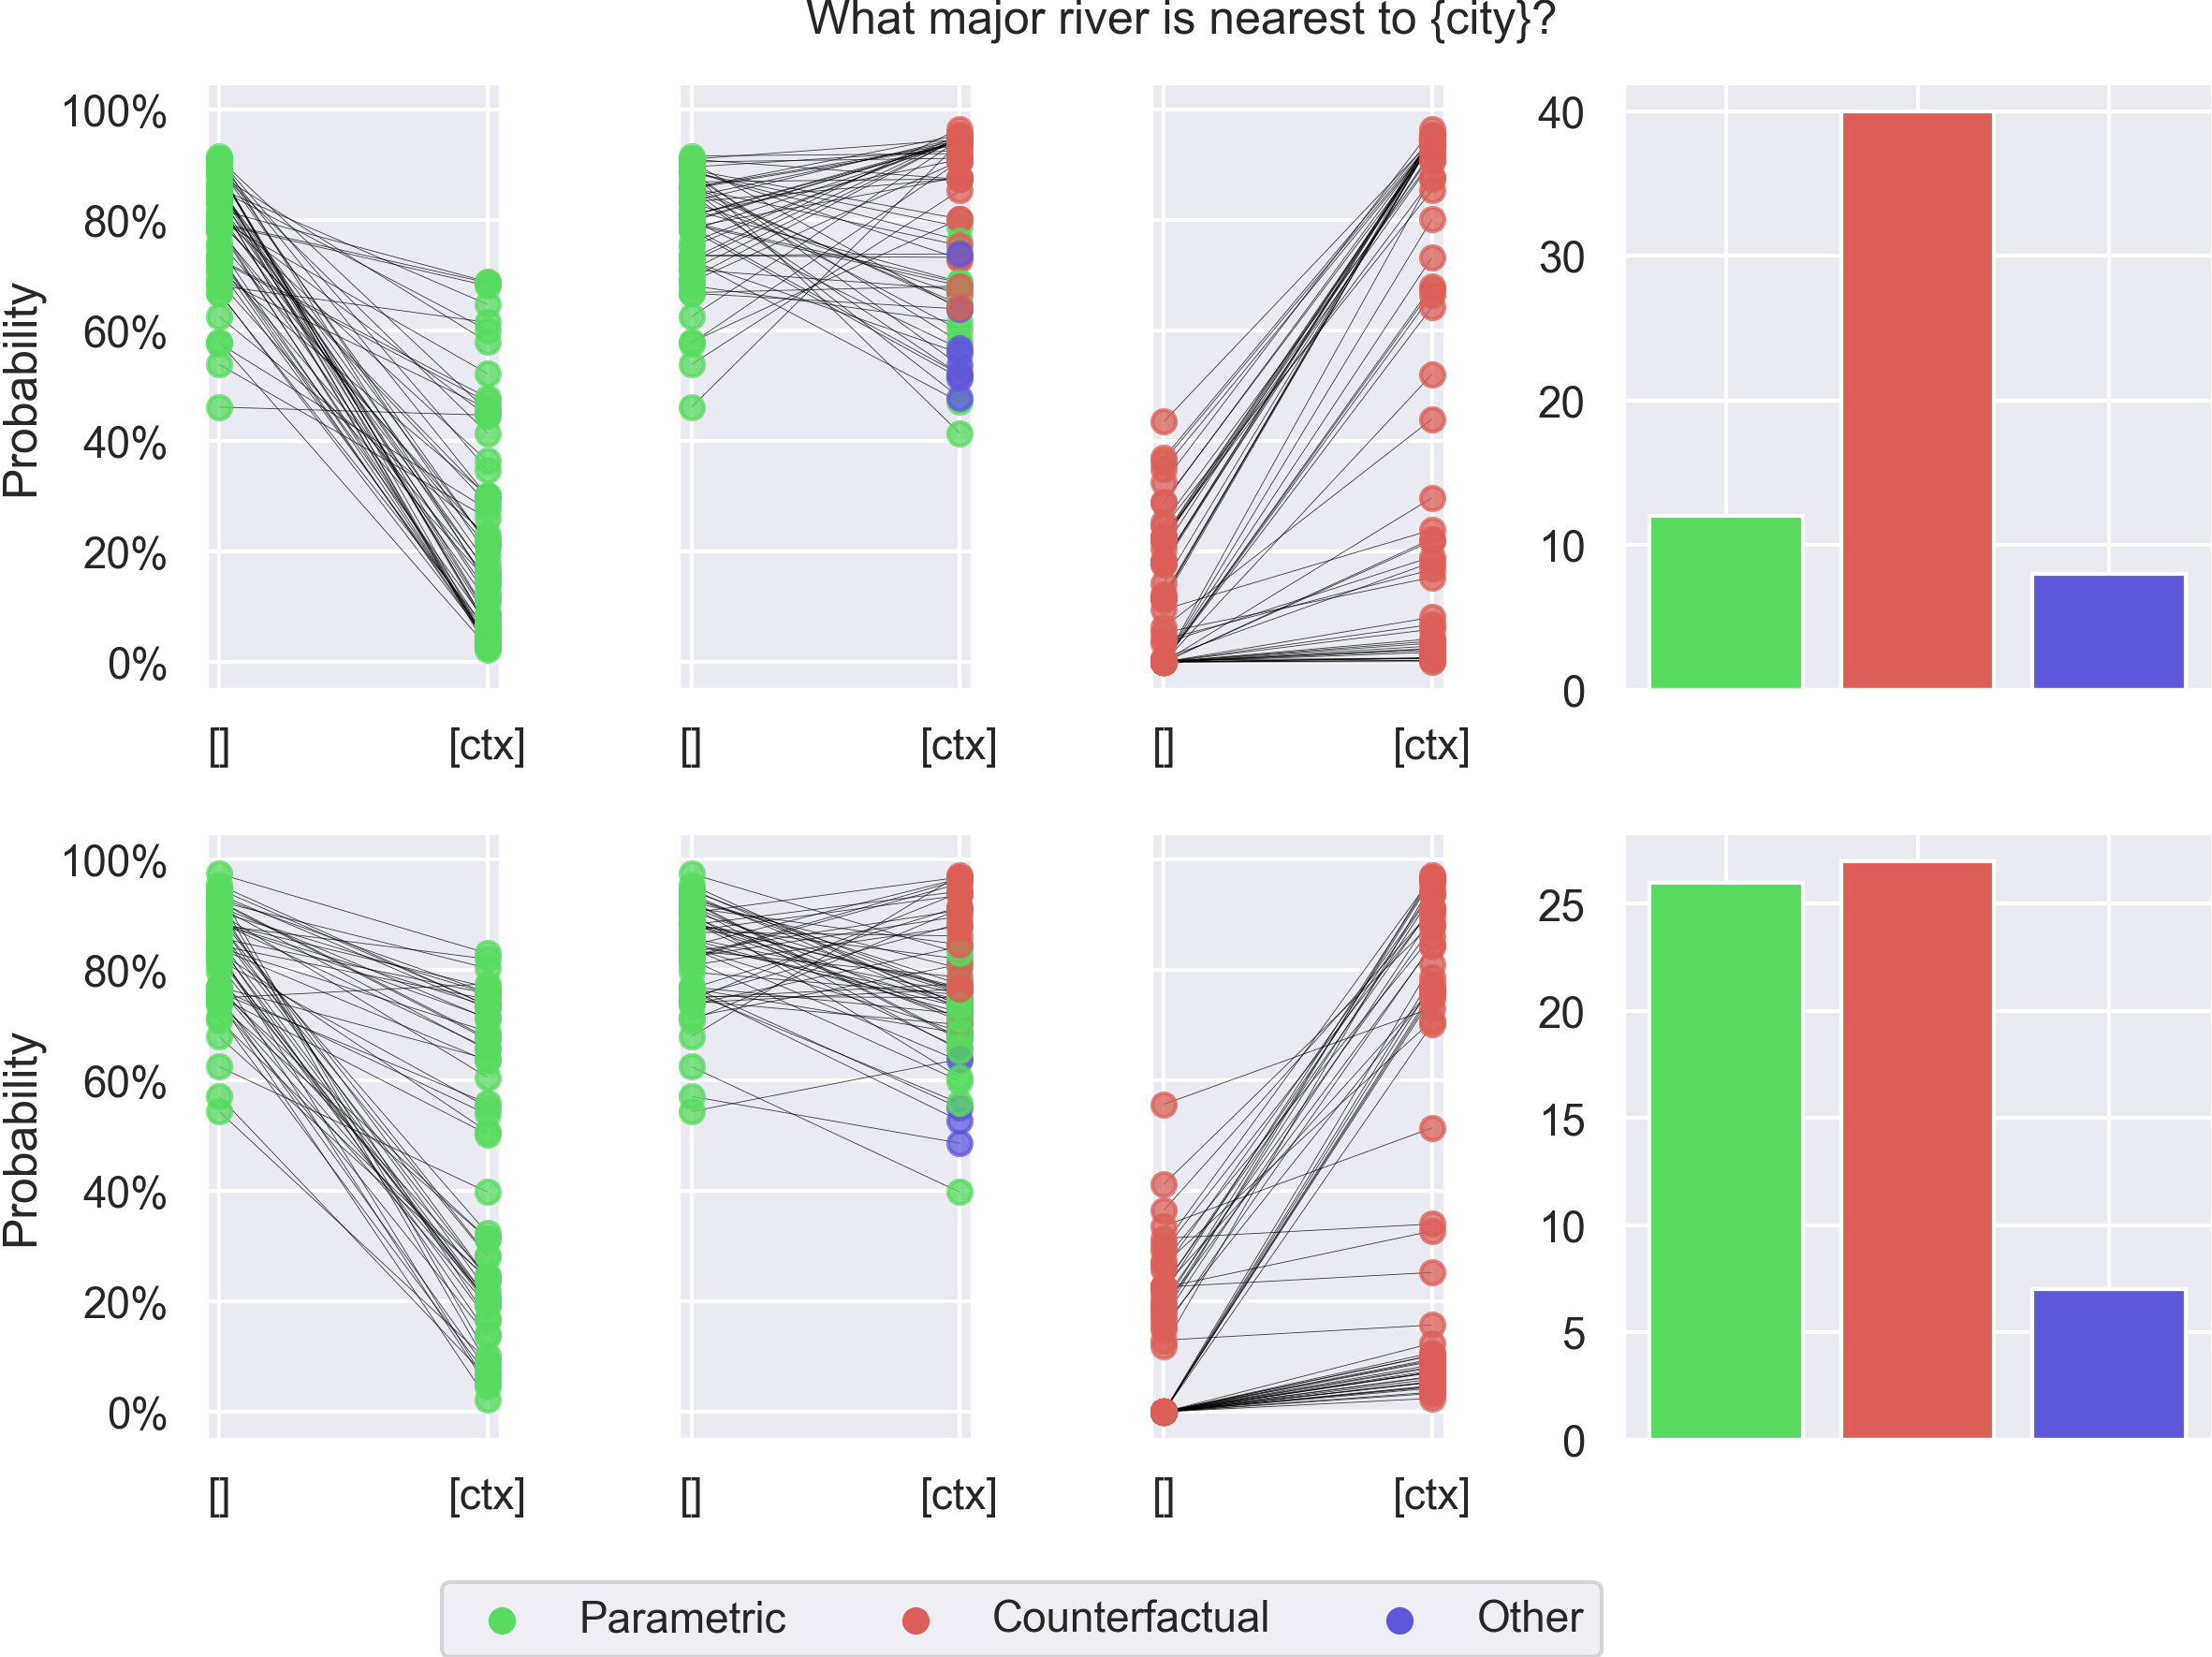
\includegraphics[width=.4\textwidth]{../figures/llama_509.png} \\[1em]
	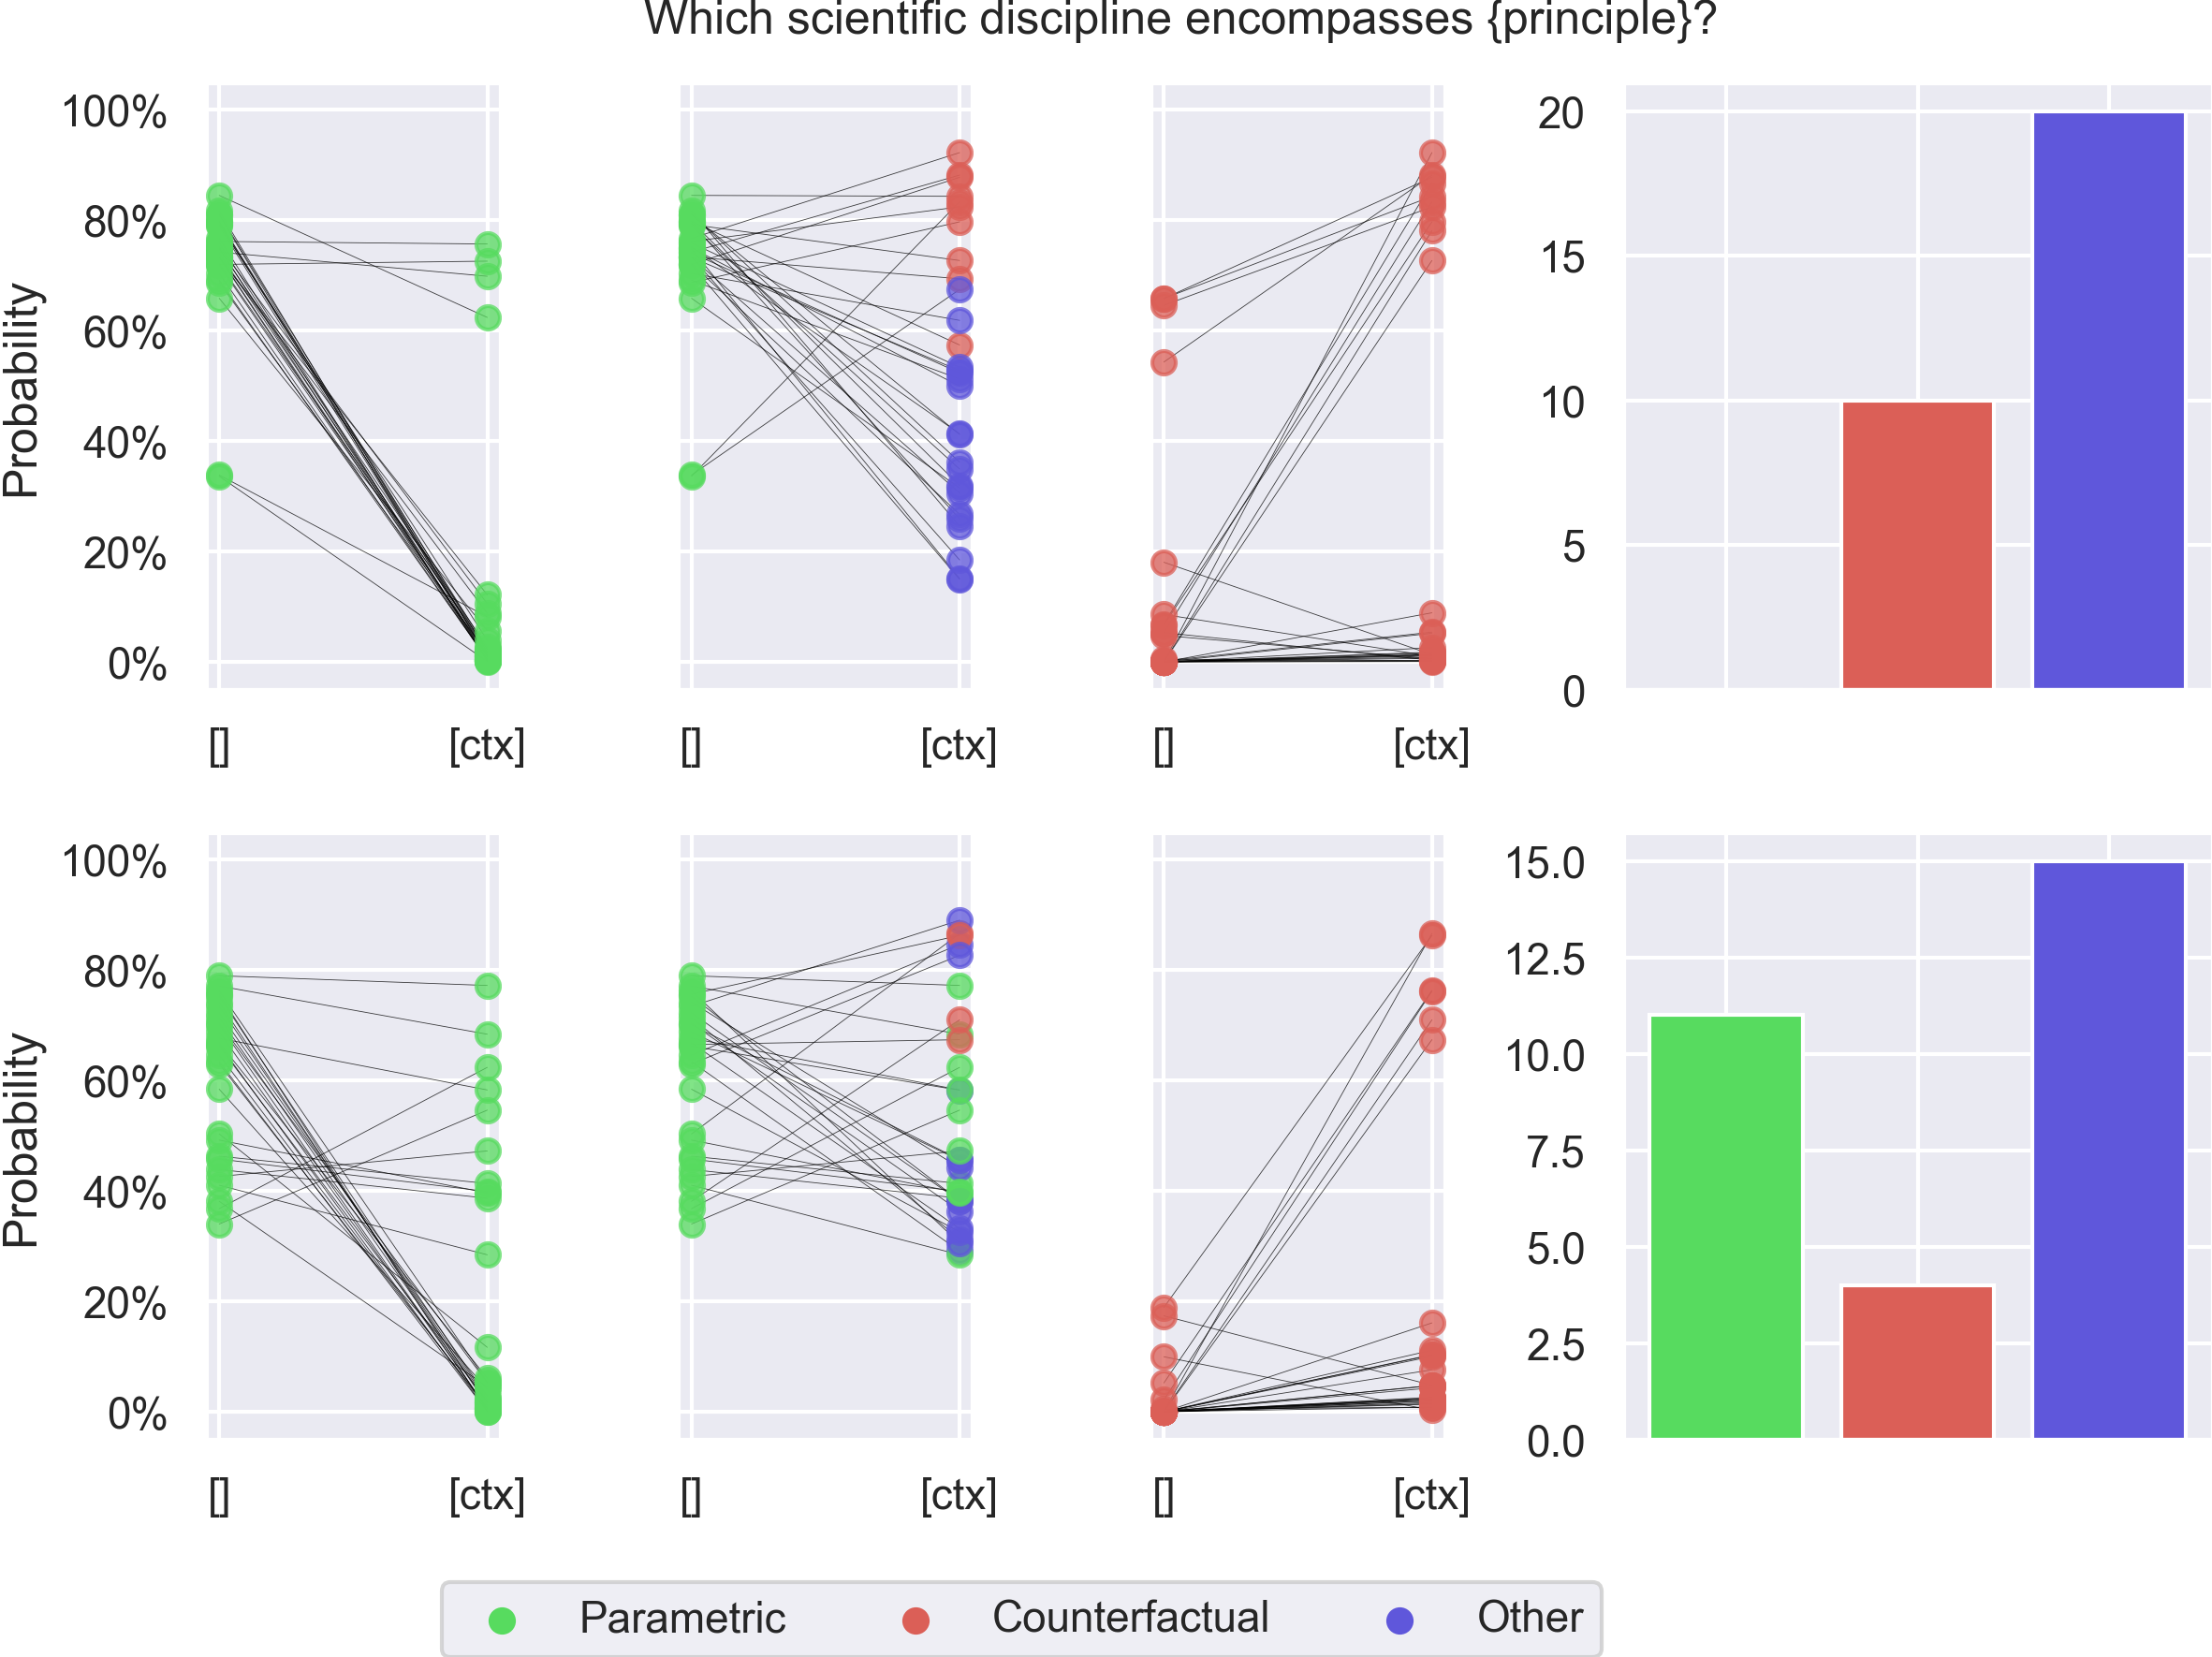
\includegraphics[width=.4\textwidth]{../figures/llama_779.png} \qquad
	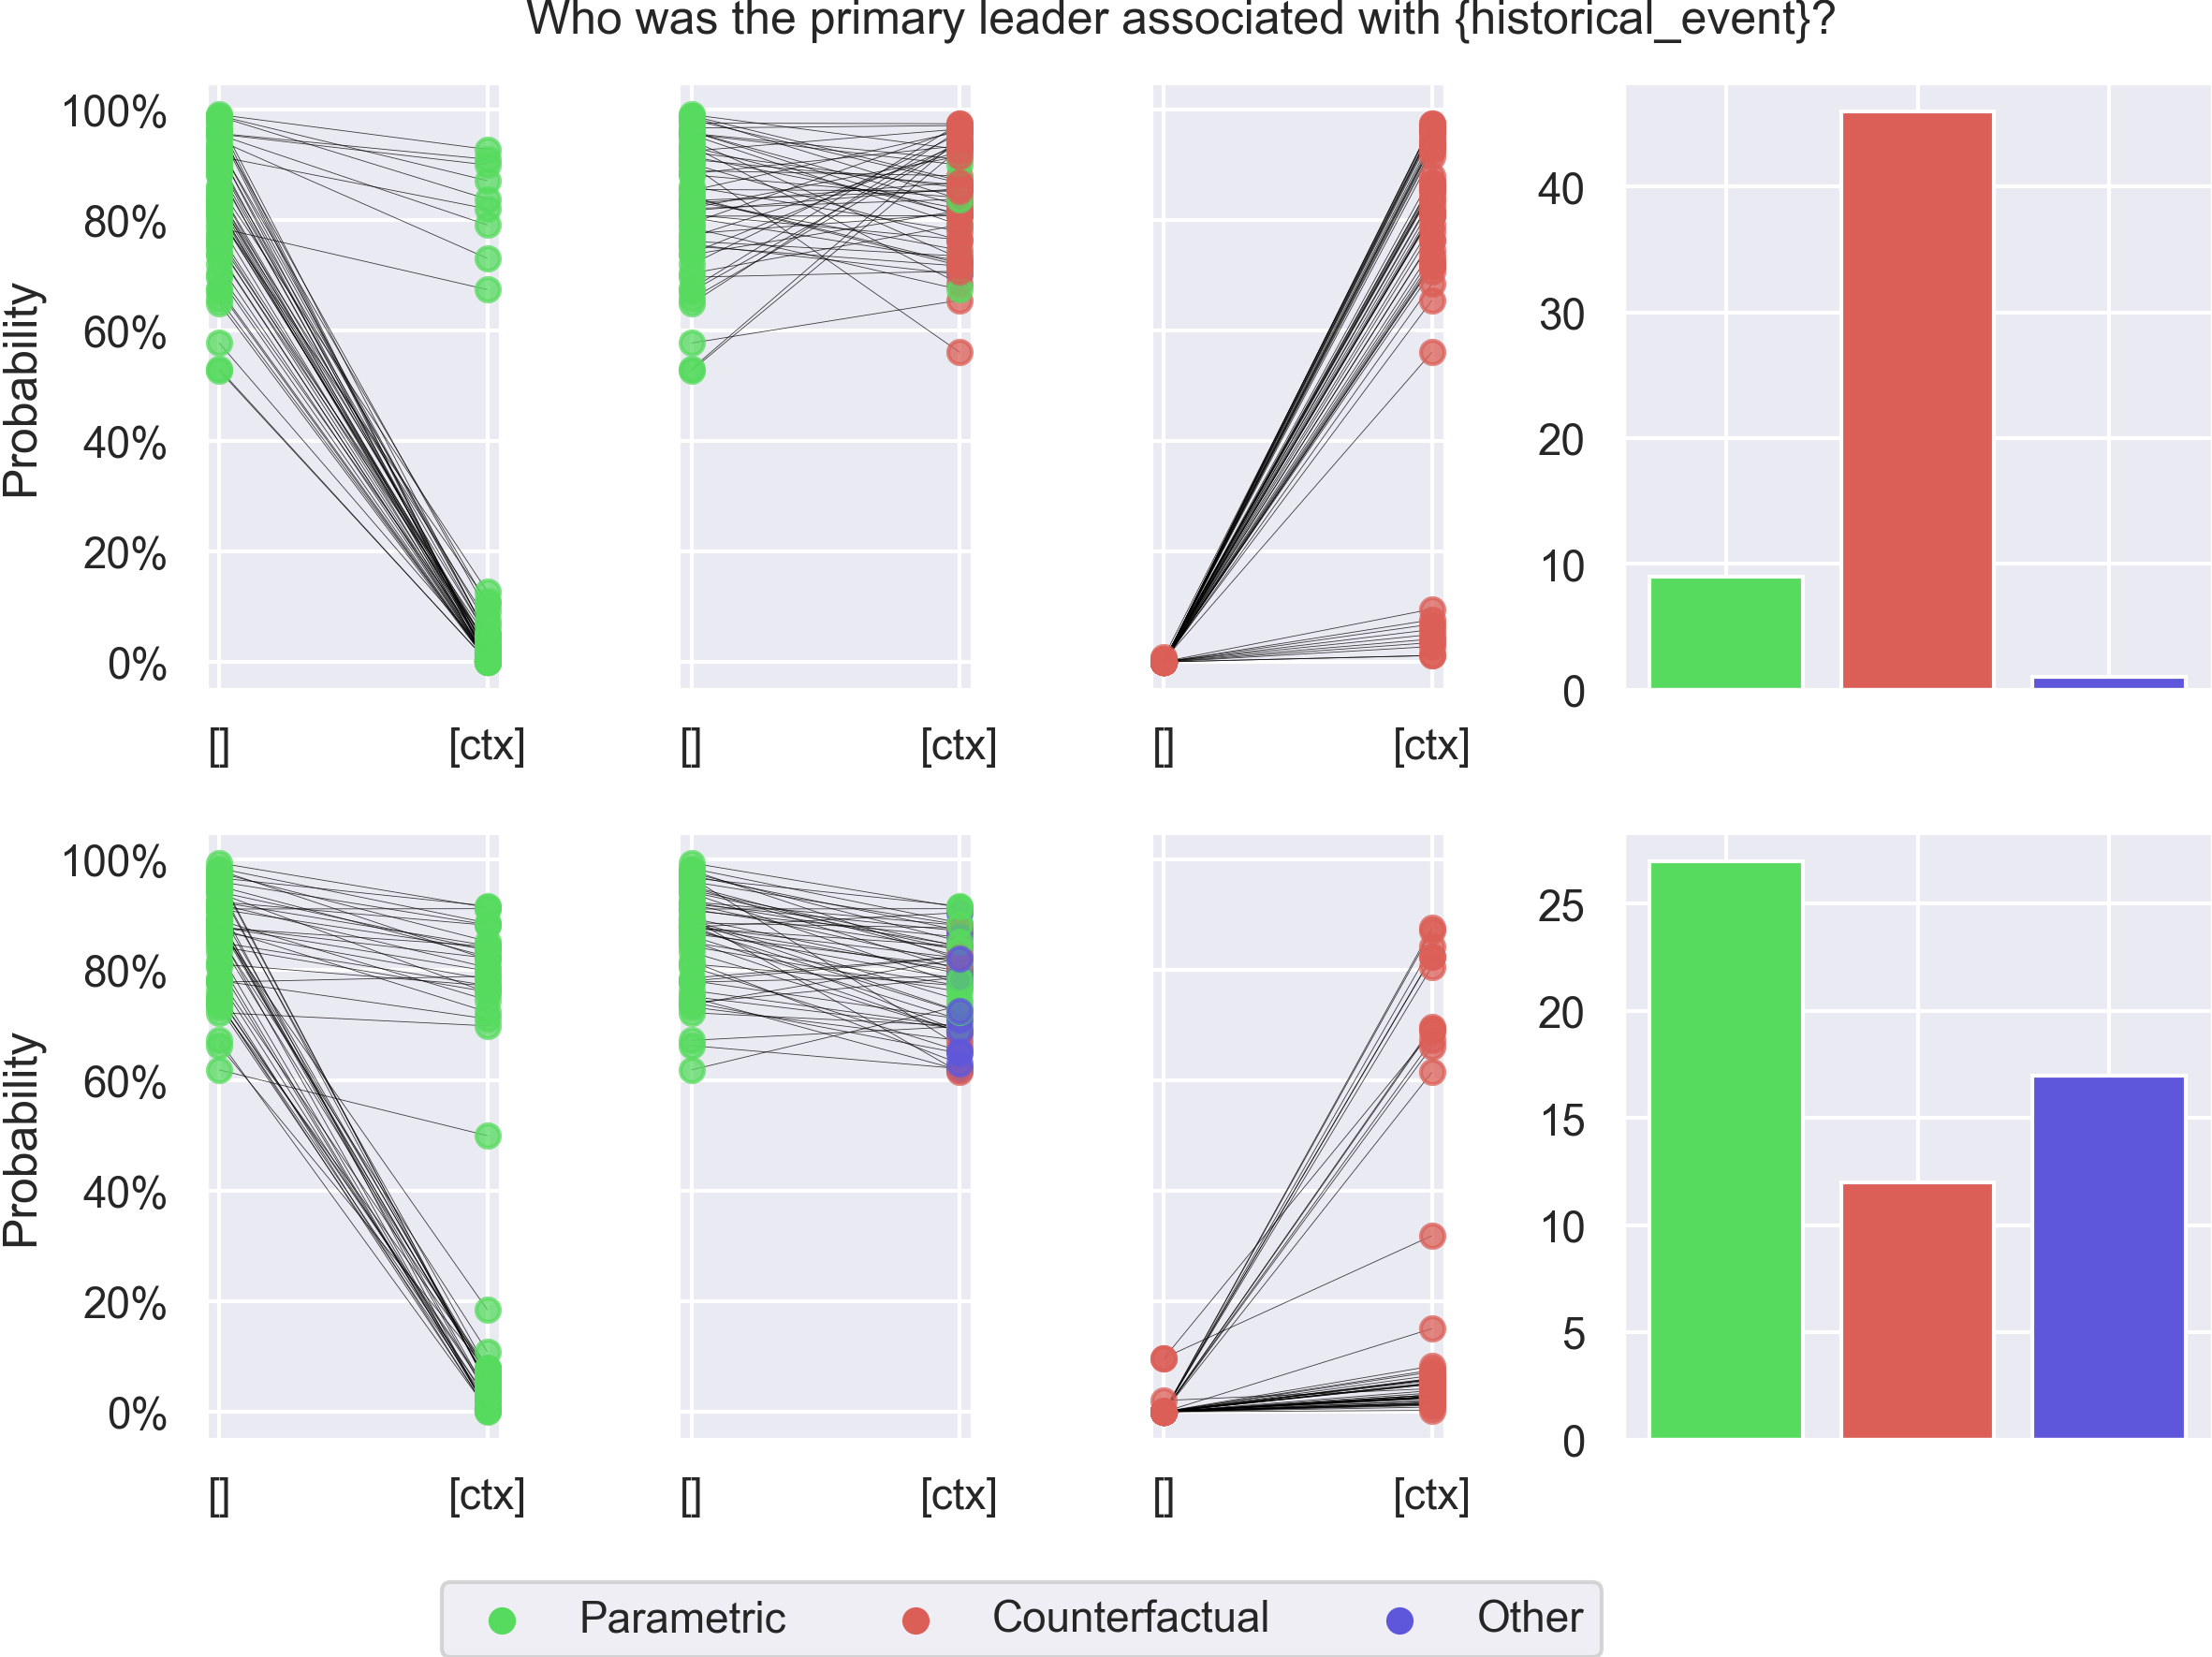
\includegraphics[width=.4\textwidth]{../figures/llama_1628.png}
\end{frame}

\begin{frame}{Some interesting results}
	Certain counterfactual answers have low probability, even when being added as part of the context.

	\vfill{}

	\centering
	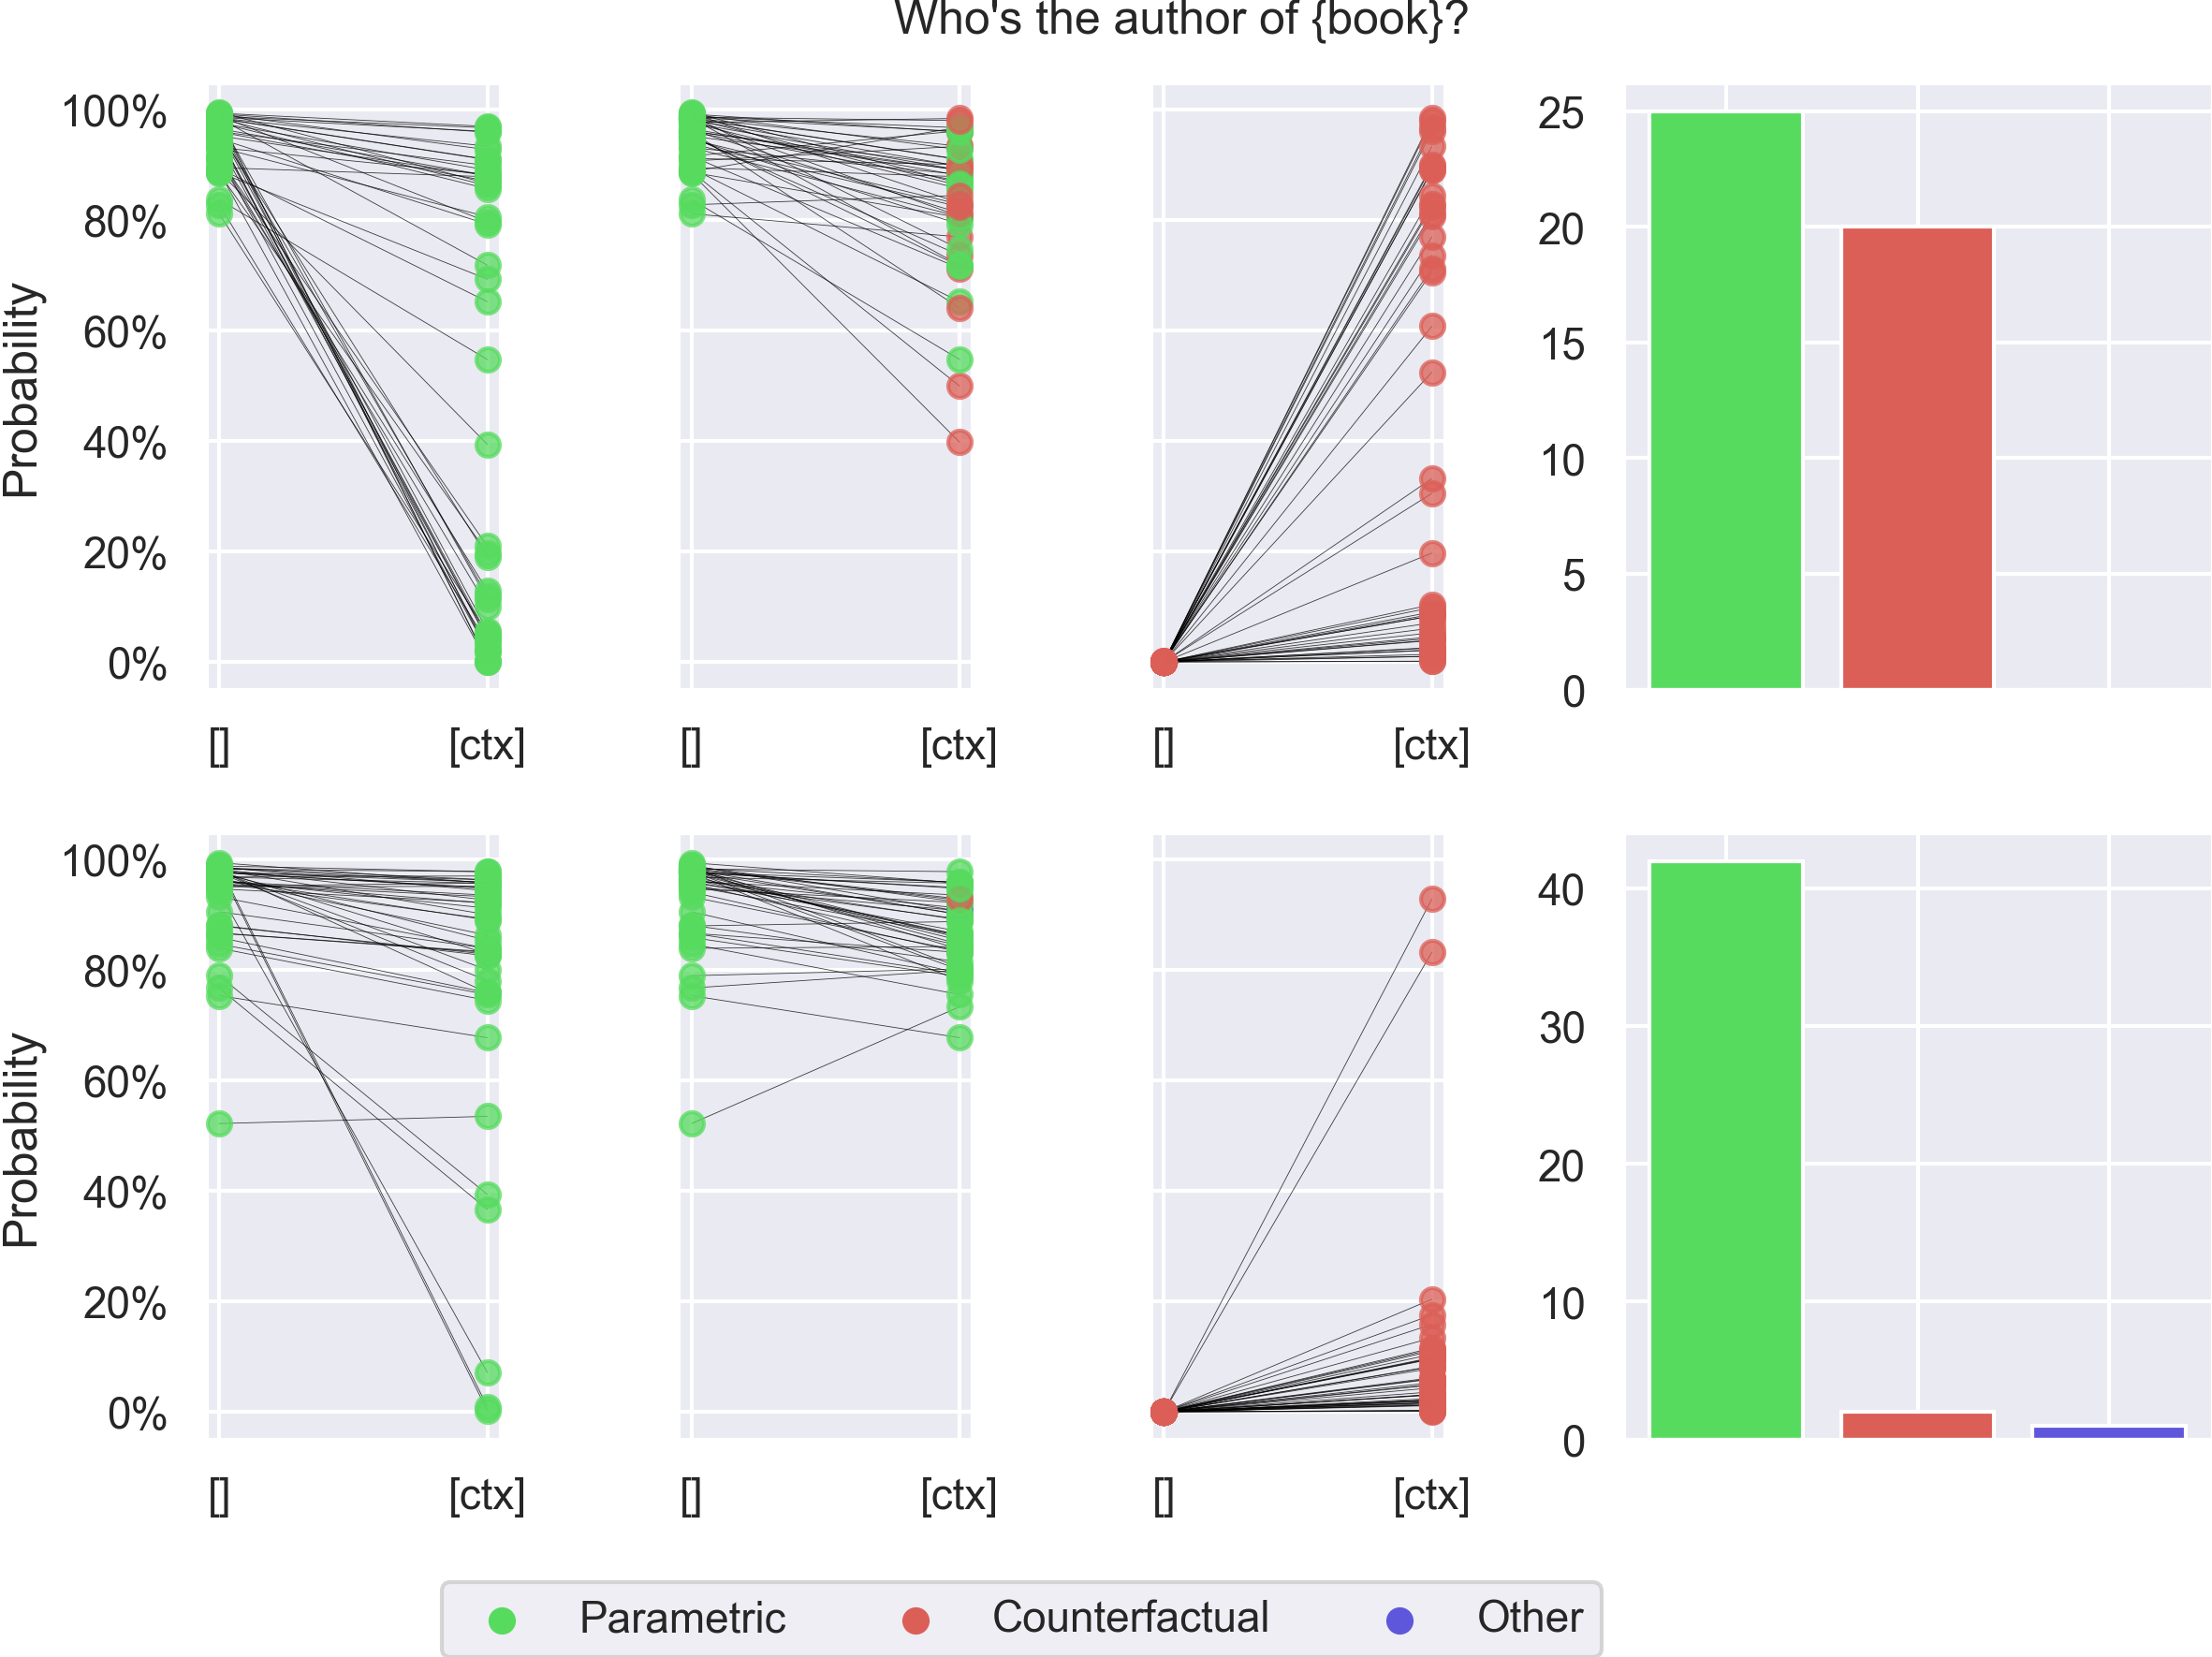
\includegraphics[width=.8\textwidth]{../figures/llama_1119.png}
\end{frame}

\section{Next Steps}
\begin{frame}{Next Steps}
	\Large
	Very important: \textbf{Define a hypothesis!}

	A lot more!
\end{frame}

\end{document}
